\documentclass[1p]{elsarticle_modified}
%\bibliographystyle{elsarticle-num}

%\usepackage[colorlinks]{hyperref}
%\usepackage{abbrmath_seonhwa} %\Abb, \Ascr, \Acal ,\Abf, \Afrak
\usepackage{amsfonts}
\usepackage{amssymb}
\usepackage{amsmath}
\usepackage{amsthm}
\usepackage{scalefnt}
\usepackage{amsbsy}
\usepackage{kotex}
\usepackage{caption}
\usepackage{subfig}
\usepackage{color}
\usepackage{graphicx}
\usepackage{xcolor} %% white, black, red, green, blue, cyan, magenta, yellow
\usepackage{float}
\usepackage{setspace}
\usepackage{hyperref}

\usepackage{tikz}
\usetikzlibrary{arrows}

\usepackage{multirow}
\usepackage{array} % fixed length table
\usepackage{hhline}

%%%%%%%%%%%%%%%%%%%%%
\makeatletter
\renewcommand*\env@matrix[1][\arraystretch]{%
	\edef\arraystretch{#1}%
	\hskip -\arraycolsep
	\let\@ifnextchar\new@ifnextchar
	\array{*\c@MaxMatrixCols c}}
\makeatother %https://tex.stackexchange.com/questions/14071/how-can-i-increase-the-line-spacing-in-a-matrix
%%%%%%%%%%%%%%%

\usepackage[normalem]{ulem}

\newcommand{\msout}[1]{\ifmmode\text{\sout{\ensuremath{#1}}}\else\sout{#1}\fi}
%SOURCE: \msout is \stkout macro in https://tex.stackexchange.com/questions/20609/strikeout-in-math-mode

\newcommand{\cancel}[1]{
	\ifmmode
	{\color{red}\msout{#1}}
	\else
	{\color{red}\sout{#1}}
	\fi
}

\newcommand{\add}[1]{
	{\color{blue}\uwave{#1}}
}

\newcommand{\replace}[2]{
	\ifmmode
	{\color{red}\msout{#1}}{\color{blue}\uwave{#2}}
	\else
	{\color{red}\sout{#1}}{\color{blue}\uwave{#2}}
	\fi
}

\newcommand{\Sol}{\mathcal{S}} %segment
\newcommand{\D}{D} %diagram
\newcommand{\A}{\mathcal{A}} %arc


%%%%%%%%%%%%%%%%%%%%%%%%%%%%%5 test

\def\sl{\operatorname{\textup{SL}}(2,\Cbb)}
\def\psl{\operatorname{\textup{PSL}}(2,\Cbb)}
\def\quan{\mkern 1mu \triangleright \mkern 1mu}

\theoremstyle{definition}
\newtheorem{thm}{Theorem}[section]
\newtheorem{prop}[thm]{Proposition}
\newtheorem{lem}[thm]{Lemma}
\newtheorem{ques}[thm]{Question}
\newtheorem{cor}[thm]{Corollary}
\newtheorem{defn}[thm]{Definition}
\newtheorem{exam}[thm]{Example}
\newtheorem{rmk}[thm]{Remark}
\newtheorem{alg}[thm]{Algorithm}

\newcommand{\I}{\sqrt{-1}}
\begin{document}

%\begin{frontmatter}
%
%\title{Boundary parabolic representations of knots up to 8 crossings}
%
%%% Group authors per affiliation:
%\author{Yunhi Cho} 
%\address{Department of Mathematics, University of Seoul, Seoul, Korea}
%\ead{yhcho@uos.ac.kr}
%
%
%\author{Seonhwa Kim} %\fnref{s_kim}}
%\address{Center for Geometry and Physics, Institute for Basic Science, Pohang, 37673, Korea}
%\ead{ryeona17@ibs.re.kr}
%
%\author{Hyuk Kim}
%\address{Department of Mathematical Sciences, Seoul National University, Seoul 08826, Korea}
%\ead{hyukkim@snu.ac.kr}
%
%\author{Seokbeom Yoon}
%\address{Department of Mathematical Sciences, Seoul National University, Seoul, 08826,  Korea}
%\ead{sbyoon15@snu.ac.kr}
%
%\begin{abstract}
%We find all boundary parabolic representation of knots up to 8 crossings.
%
%\end{abstract}
%\begin{keyword}
%    \MSC[2010] 57M25 
%\end{keyword}
%
%\end{frontmatter}

%\linenumbers
%\tableofcontents
%
\newcommand\colored[1]{\textcolor{white}{\rule[-0.35ex]{0.8em}{1.4ex}}\kern-0.8em\color{red} #1}%
%\newcommand\colored[1]{\textcolor{white}{ #1}\kern-2.17ex	\textcolor{white}{ #1}\kern-1.81ex	\textcolor{white}{ #1}\kern-2.15ex\color{red}#1	}

{\Large $\underline{12n_{0432}~(K12n_{0432})}$}

\setlength{\tabcolsep}{10pt}
\renewcommand{\arraystretch}{1.6}
\vspace{1cm}\begin{tabular}{m{100pt}>{\centering\arraybackslash}m{274pt}}
\multirow{5}{120pt}{
	\centering
	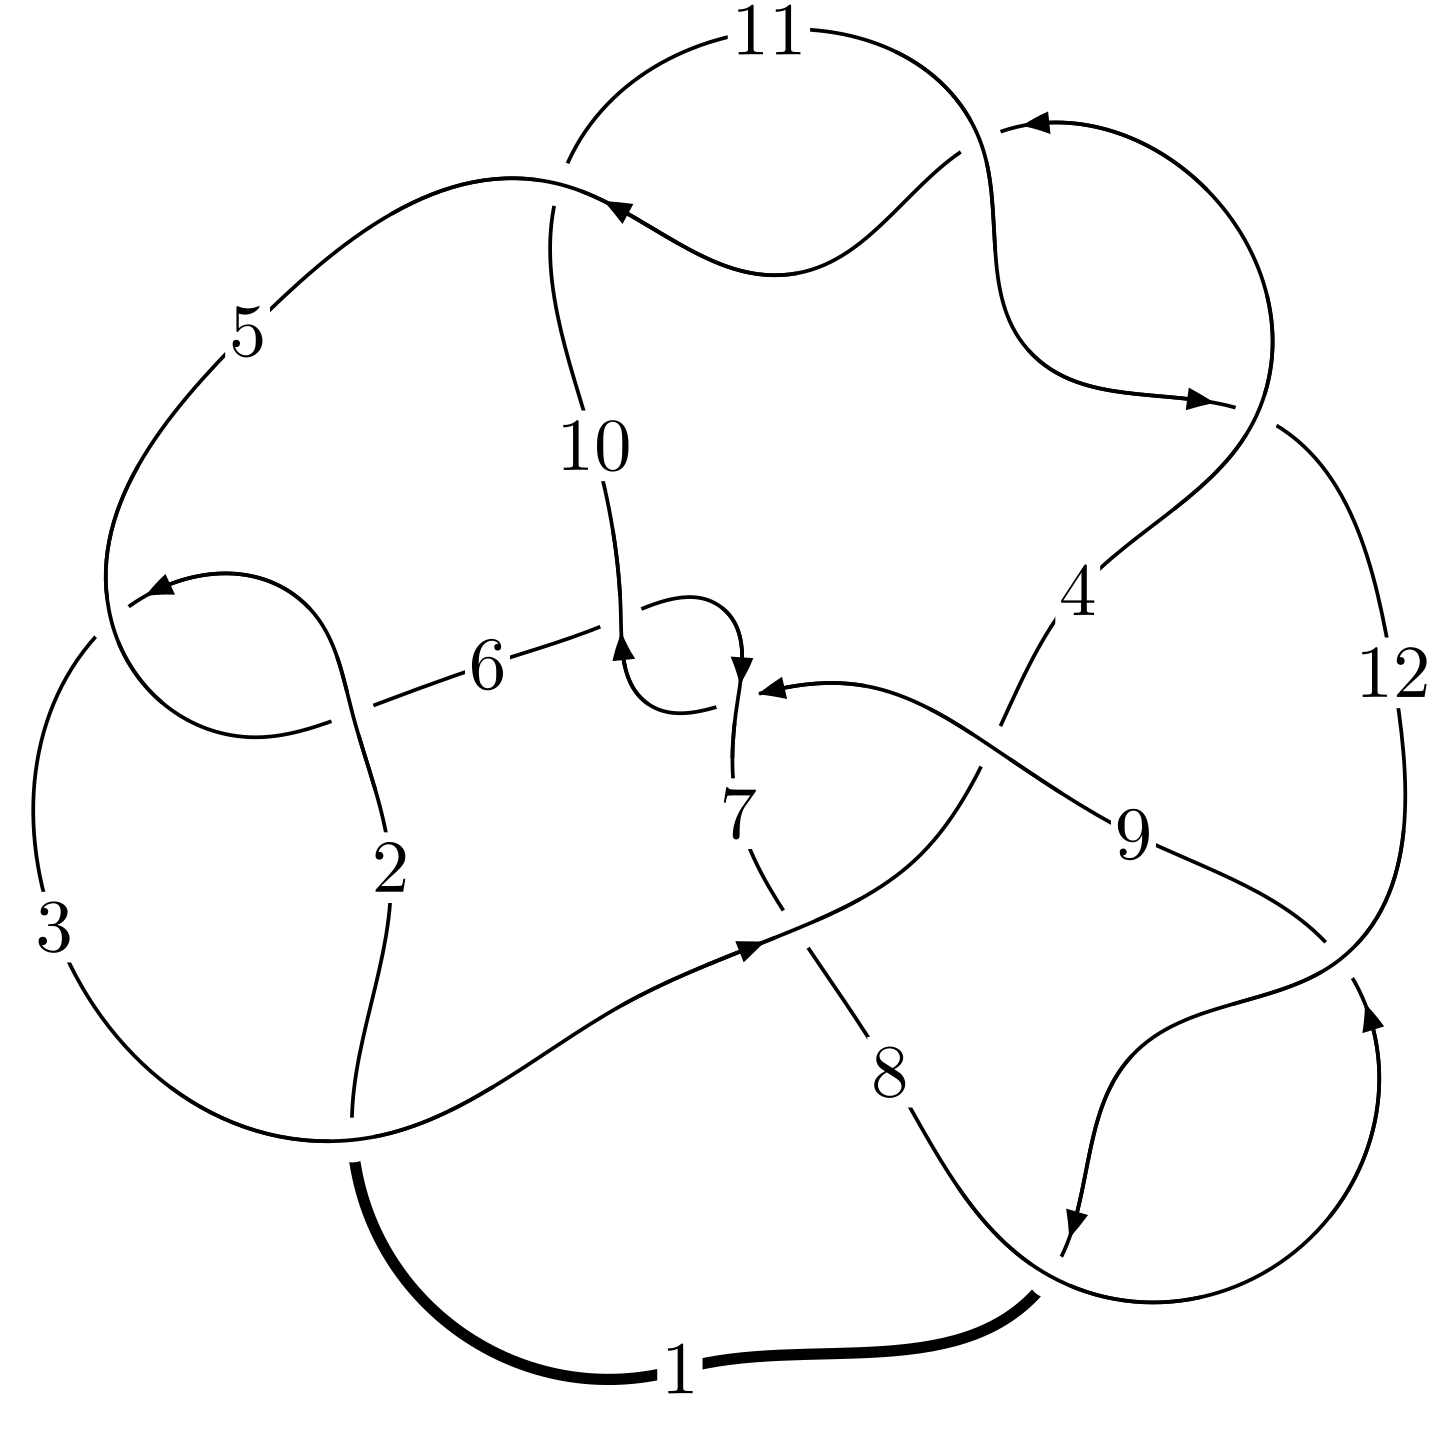
\includegraphics[width=112pt]{../../../GIT/diagram.site/Diagrams/png/2521_12n_0432.png}\\
\ \ \ A knot diagram\footnotemark}&
\allowdisplaybreaks
\textbf{Linearized knot diagam} \\
\cline{2-2}
 &
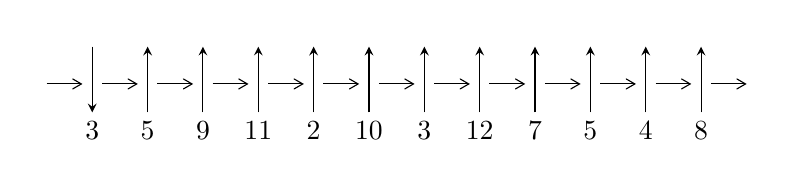
\begin{tikzpicture}[x=20pt, y=17pt]
	% nodes
	\node (C0) at (0, 0) {};
	\node (C1) at (1, 0) {};
	\node (C1U) at (1, +1) {};
	\node (C1D) at (1, -1) {3};

	\node (C2) at (2, 0) {};
	\node (C2U) at (2, +1) {};
	\node (C2D) at (2, -1) {5};

	\node (C3) at (3, 0) {};
	\node (C3U) at (3, +1) {};
	\node (C3D) at (3, -1) {9};

	\node (C4) at (4, 0) {};
	\node (C4U) at (4, +1) {};
	\node (C4D) at (4, -1) {11};

	\node (C5) at (5, 0) {};
	\node (C5U) at (5, +1) {};
	\node (C5D) at (5, -1) {2};

	\node (C6) at (6, 0) {};
	\node (C6U) at (6, +1) {};
	\node (C6D) at (6, -1) {10};

	\node (C7) at (7, 0) {};
	\node (C7U) at (7, +1) {};
	\node (C7D) at (7, -1) {3};

	\node (C8) at (8, 0) {};
	\node (C8U) at (8, +1) {};
	\node (C8D) at (8, -1) {12};

	\node (C9) at (9, 0) {};
	\node (C9U) at (9, +1) {};
	\node (C9D) at (9, -1) {7};

	\node (C10) at (10, 0) {};
	\node (C10U) at (10, +1) {};
	\node (C10D) at (10, -1) {5};

	\node (C11) at (11, 0) {};
	\node (C11U) at (11, +1) {};
	\node (C11D) at (11, -1) {4};

	\node (C12) at (12, 0) {};
	\node (C12U) at (12, +1) {};
	\node (C12D) at (12, -1) {8};
	\node (C13) at (13, 0) {};

	% arrows
	\draw[->,>={angle 60}]
	(C0) edge (C1) (C1) edge (C2) (C2) edge (C3) (C3) edge (C4) (C4) edge (C5) (C5) edge (C6) (C6) edge (C7) (C7) edge (C8) (C8) edge (C9) (C9) edge (C10) (C10) edge (C11) (C11) edge (C12) (C12) edge (C13) ;	\draw[->,>=stealth]
	(C1U) edge (C1D) (C2D) edge (C2U) (C3D) edge (C3U) (C4D) edge (C4U) (C5D) edge (C5U) (C6D) edge (C6U) (C7D) edge (C7U) (C8D) edge (C8U) (C9D) edge (C9U) (C10D) edge (C10U) (C11D) edge (C11U) (C12D) edge (C12U) ;
	\end{tikzpicture} \\
\hhline{~~} \\& 
\textbf{Solving Sequence} \\ \cline{2-2} 
 &
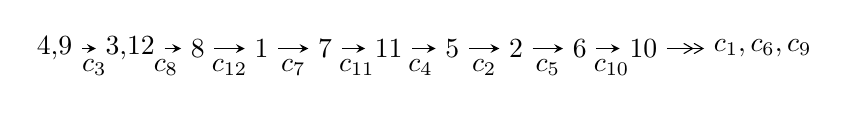
\begin{tikzpicture}[x=23pt, y=7pt]
	% node
	\node (A0) at (-1/8, 0) {4,9};
	\node (A1) at (17/16, 0) {3,12};
	\node (A2) at (17/8, 0) {8};
	\node (A3) at (25/8, 0) {1};
	\node (A4) at (33/8, 0) {7};
	\node (A5) at (41/8, 0) {11};
	\node (A6) at (49/8, 0) {5};
	\node (A7) at (57/8, 0) {2};
	\node (A8) at (65/8, 0) {6};
	\node (A9) at (73/8, 0) {10};
	\node (C1) at (1/2, -1) {$c_{3}$};
	\node (C2) at (13/8, -1) {$c_{8}$};
	\node (C3) at (21/8, -1) {$c_{12}$};
	\node (C4) at (29/8, -1) {$c_{7}$};
	\node (C5) at (37/8, -1) {$c_{11}$};
	\node (C6) at (45/8, -1) {$c_{4}$};
	\node (C7) at (53/8, -1) {$c_{2}$};
	\node (C8) at (61/8, -1) {$c_{5}$};
	\node (C9) at (69/8, -1) {$c_{10}$};
	\node (A10) at (11, 0) {$c_{1},c_{6},c_{9}$};

	% edge
	\draw[->,>=stealth]	
	(A0) edge (A1) (A1) edge (A2) (A2) edge (A3) (A3) edge (A4) (A4) edge (A5) (A5) edge (A6) (A6) edge (A7) (A7) edge (A8) (A8) edge (A9) ;
	\draw[->>,>={angle 60}]	
	(A9) edge (A10);
\end{tikzpicture} \\ 

\end{tabular} \\

\footnotetext{
The image of knot diagram is generated by the software ``\textbf{Draw programme}" developed by Andrew Bartholomew(\url{http://www.layer8.co.uk/maths/draw/index.htm\#Running-draw}), where we modified some parts for our purpose(\url{https://github.com/CATsTAILs/LinksPainter}).
}\phantom \\ \newline 
\centering \textbf{Ideals for irreducible components\footnotemark of $X_{\text{par}}$} 
 
\begin{align*}
I^u_{1}&=\langle 
74 u^{12}-692 u^{11}+\cdots+2529 b+2355,\;785 u^{12}-3703 u^{11}+\cdots+7587 a+387,\\
\phantom{I^u_{1}}&\phantom{= \langle  }u^{13}-5 u^{12}+15 u^{11}-29 u^{10}+44 u^9-54 u^8+61 u^7-62 u^6+65 u^5-67 u^4+72 u^3-57 u^2+36 u-9\rangle \\
I^u_{2}&=\langle 
b+u-1,\;u^4-4 u^3+8 u^2+a-7 u+3,\;u^5-4 u^4+8 u^3-7 u^2+2 u+1\rangle \\
I^u_{3}&=\langle 
a^3- a^2 u- a^2+3 a u+b+2 u+3,\;a^4- a^3 u+2 a^2 u- a^2+4 a u+3 a+2,\;u^2+u+1\rangle \\
I^u_{4}&=\langle 
- a^3- a^2 u- a^2+a u+b+2 u+1,\;a^4+a^3 u-2 a^2 u- a^2-2 a u- a+2 u,\;u^2+u+1\rangle \\
\\
\end{align*}
\raggedright * 4 irreducible components of $\dim_{\mathbb{C}}=0$, with total 34 representations.\\
\footnotetext{All coefficients of polynomials are rational numbers. But the coefficients are sometimes approximated in decimal forms when there is not enough margin.}
\newpage
\renewcommand{\arraystretch}{1}
\centering \section*{I. $I^u_{1}= \langle 74 u^{12}-692 u^{11}+\cdots+2529 b+2355,\;785 u^{12}-3703 u^{11}+\cdots+7587 a+387,\;u^{13}-5 u^{12}+\cdots+36 u-9 \rangle$}
\flushleft \textbf{(i) Arc colorings}\\
\begin{tabular}{m{7pt} m{180pt} m{7pt} m{180pt} }
\flushright $a_{4}=$&$\begin{pmatrix}1\\0\end{pmatrix}$ \\
\flushright $a_{9}=$&$\begin{pmatrix}0\\u\end{pmatrix}$ \\
\flushright $a_{3}=$&$\begin{pmatrix}1\\u^2\end{pmatrix}$ \\
\flushright $a_{12}=$&$\begin{pmatrix}-0.103466 u^{12}+0.488072 u^{11}+\cdots+2.94108 u-0.0510083\\-0.0292606 u^{12}+0.273626 u^{11}+\cdots+3.67378 u-0.931198\end{pmatrix}$ \\
\flushright $a_{8}=$&$\begin{pmatrix}-0.0726242 u^{12}+0.196652 u^{11}+\cdots-1.94029 u+0.651246\\-0.166469 u^{12}+0.622776 u^{11}+\cdots+4.26572 u-0.653618\end{pmatrix}$ \\
\flushright $a_{1}=$&$\begin{pmatrix}0.168051 u^{12}-0.640569 u^{11}+\cdots-3.47331 u+1.42467\\0.0723606 u^{12}-0.397390 u^{11}+\cdots-4.74733 u+1.77580\end{pmatrix}$ \\
\flushright $a_{7}=$&$\begin{pmatrix}-0.115724 u^{12}+0.320417 u^{11}+\cdots-0.866746 u-0.193357\\-0.148675 u^{12}+1.00593 u^{11}+\cdots+7.18031 u-1.47924\end{pmatrix}$ \\
\flushright $a_{11}=$&$\begin{pmatrix}-0.0742059 u^{12}+0.214446 u^{11}+\cdots-0.732701 u+0.880190\\-0.0292606 u^{12}+0.273626 u^{11}+\cdots+3.67378 u-0.931198\end{pmatrix}$ \\
\flushright $a_{5}=$&$\begin{pmatrix}0.0938447 u^{12}-0.426124 u^{11}+\cdots-5.20601 u+2.30486\\-0.166469 u^{12}+0.622776 u^{11}+\cdots+3.26572 u-0.653618\end{pmatrix}$ \\
\flushright $a_{2}=$&$\begin{pmatrix}0.319889 u^{12}-1.34875 u^{11}+\cdots-4.40214 u+1.44603\\-0.329775 u^{12}+0.876631 u^{11}+\cdots-5.21708 u+2.23488\end{pmatrix}$ \\
\flushright $a_{6}=$&$\begin{pmatrix}0.628312 u^{12}-2.59628 u^{11}+\cdots-11.5492 u+3.46856\\-0.758798 u^{12}+2.67537 u^{11}+\cdots+5.17556 u-0.747331\end{pmatrix}$ \\
\flushright $a_{10}=$&$\begin{pmatrix}-0.00237248 u^{12}-0.139976 u^{11}+\cdots-2.52195 u+0.843416\\0.199684 u^{12}-0.774219 u^{11}+\cdots-4.62515 u+1.51246\end{pmatrix}$\\&\end{tabular}
\flushleft \textbf{(ii) Obstruction class $= -1$}\\~\\
\flushleft \textbf{(iii) Cusp Shapes $= \frac{3325}{2529} u^{12}-\frac{17666}{2529} u^{11}+\frac{17227}{843} u^{10}-\frac{96773}{2529} u^9+\frac{137357}{2529} u^8-\frac{17822}{281} u^7+\frac{173059}{2529} u^6-\frac{170021}{2529} u^5+\frac{175199}{2529} u^4-\frac{187657}{2529} u^3+\frac{67681}{843} u^2-\frac{48875}{843} u+\frac{9022}{281}$}\\~\\
\newpage\renewcommand{\arraystretch}{1}
\flushleft \textbf{(iv) u-Polynomials at the component}\newline \\
\begin{tabular}{m{50pt}|m{274pt}}
Crossings & \hspace{64pt}u-Polynomials at each crossing \\
\hline $$\begin{aligned}c_{1}\end{aligned}$$&$\begin{aligned}
&u^{13}- u^{12}+\cdots+4 u-1
\end{aligned}$\\
\hline $$\begin{aligned}c_{2},c_{5},c_{6}\\c_{9}\end{aligned}$$&$\begin{aligned}
&u^{13}+u^{12}+\cdots+2 u-1
\end{aligned}$\\
\hline $$\begin{aligned}c_{3}\end{aligned}$$&$\begin{aligned}
&u^{13}-5 u^{12}+\cdots+36 u-9
\end{aligned}$\\
\hline $$\begin{aligned}c_{4},c_{8},c_{10}\\c_{11},c_{12}\end{aligned}$$&$\begin{aligned}
&u^{13}+8 u^{11}+\cdots- u-1
\end{aligned}$\\
\hline $$\begin{aligned}c_{7}\end{aligned}$$&$\begin{aligned}
&u^{13}- u^{12}+\cdots+90 u-25
\end{aligned}$\\
\hline
\end{tabular}\\~\\
\newpage\renewcommand{\arraystretch}{1}
\flushleft \textbf{(v) Riley Polynomials at the component}\newline \\
\begin{tabular}{m{50pt}|m{274pt}}
Crossings & \hspace{64pt}Riley Polynomials at each crossing \\
\hline $$\begin{aligned}c_{1}\end{aligned}$$&$\begin{aligned}
&y^{13}+35 y^{12}+\cdots+212 y-1
\end{aligned}$\\
\hline $$\begin{aligned}c_{2},c_{5},c_{6}\\c_{9}\end{aligned}$$&$\begin{aligned}
&y^{13}- y^{12}+\cdots+4 y-1
\end{aligned}$\\
\hline $$\begin{aligned}c_{3}\end{aligned}$$&$\begin{aligned}
&y^{13}+5 y^{12}+\cdots+270 y-81
\end{aligned}$\\
\hline $$\begin{aligned}c_{4},c_{8},c_{10}\\c_{11},c_{12}\end{aligned}$$&$\begin{aligned}
&y^{13}+16 y^{12}+\cdots-5 y-1
\end{aligned}$\\
\hline $$\begin{aligned}c_{7}\end{aligned}$$&$\begin{aligned}
&y^{13}-7 y^{12}+\cdots+3150 y-625
\end{aligned}$\\
\hline
\end{tabular}\\~\\
\newpage\flushleft \textbf{(vi) Complex Volumes and Cusp Shapes}
$$\begin{array}{c|c|c}  
\text{Solutions to }I^u_{1}& \I (\text{vol} + \sqrt{-1}CS) & \text{Cusp shape}\\
 \hline 
\begin{aligned}
u &= \phantom{-}0.377421 + 0.995561 I \\
a &= \phantom{-}1.42395 + 0.27192 I \\
b &= \phantom{-}0.26672 + 1.52025 I\end{aligned}
 & -13.25130 + 1.59234 I & -1.196156 - 0.103558 I \\ \hline\begin{aligned}
u &= \phantom{-}0.377421 - 0.995561 I \\
a &= \phantom{-}1.42395 - 0.27192 I \\
b &= \phantom{-}0.26672 - 1.52025 I\end{aligned}
 & -13.25130 - 1.59234 I & -1.196156 + 0.103558 I \\ \hline\begin{aligned}
u &= -0.826366 + 0.684268 I \\
a &= -0.040776 + 0.277567 I \\
b &= -0.156234 - 0.257273 I\end{aligned}
 & -1.74296 - 2.47632 I & \phantom{-}11.79558 + 3.97407 I \\ \hline\begin{aligned}
u &= -0.826366 - 0.684268 I \\
a &= -0.040776 - 0.277567 I \\
b &= -0.156234 + 0.257273 I\end{aligned}
 & -1.74296 + 2.47632 I & \phantom{-}11.79558 - 3.97407 I \\ \hline\begin{aligned}
u &= -0.261323 + 1.190470 I \\
a &= -0.753030 + 0.372533 I \\
b &= -0.246705 - 0.993811 I\end{aligned}
 & -5.78672 - 1.79985 I & \phantom{-}0.24328 + 2.30841 I \\ \hline\begin{aligned}
u &= -0.261323 - 1.190470 I \\
a &= -0.753030 - 0.372533 I \\
b &= -0.246705 + 0.993811 I\end{aligned}
 & -5.78672 + 1.79985 I & \phantom{-}0.24328 - 2.30841 I \\ \hline\begin{aligned}
u &= \phantom{-}1.197260 + 0.637614 I \\
a &= \phantom{-}0.000701 + 1.040290 I \\
b &= -0.662461 + 1.245930 I\end{aligned}
 & \phantom{-}3.92798 - 4.17113 I & \phantom{-}7.23672 + 2.38066 I \\ \hline\begin{aligned}
u &= \phantom{-}1.197260 - 0.637614 I \\
a &= \phantom{-}0.000701 - 1.040290 I \\
b &= -0.662461 - 1.245930 I\end{aligned}
 & \phantom{-}3.92798 + 4.17113 I & \phantom{-}7.23672 - 2.38066 I \\ \hline\begin{aligned}
u &= \phantom{-}0.80433 + 1.22011 I \\
a &= \phantom{-}1.250130 + 0.103984 I \\
b &= \phantom{-}0.87865 + 1.60894 I\end{aligned}
 & \phantom{-}1.94166 + 11.33090 I & \phantom{-}6.29855 - 5.31818 I \\ \hline\begin{aligned}
u &= \phantom{-}0.80433 - 1.22011 I \\
a &= \phantom{-}1.250130 - 0.103984 I \\
b &= \phantom{-}0.87865 - 1.60894 I\end{aligned}
 & \phantom{-}1.94166 - 11.33090 I & \phantom{-}6.29855 + 5.31818 I\\
 \hline 
 \end{array}$$\newpage$$\begin{array}{c|c|c}  
\text{Solutions to }I^u_{1}& \I (\text{vol} + \sqrt{-1}CS) & \text{Cusp shape}\\
 \hline 
\begin{aligned}
u &= \phantom{-}0.425591\phantom{ +0.000000I} \\
a &= \phantom{-}0.763681\phantom{ +0.000000I} \\
b &= \phantom{-}0.325016\phantom{ +0.000000I}\end{aligned}
 & \phantom{-}0.561978\phantom{ +0.000000I} & \phantom{-}17.8790\phantom{ +0.000000I} \\ \hline\begin{aligned}
u &= \phantom{-}0.99588 + 1.33587 I \\
a &= -0.762815 - 0.387161 I \\
b &= -0.24248 - 1.40459 I\end{aligned}
 & -8.39874 + 4.39673 I & \phantom{-}4.68261 + 1.52874 I \\ \hline\begin{aligned}
u &= \phantom{-}0.99588 - 1.33587 I \\
a &= -0.762815 + 0.387161 I \\
b &= -0.24248 + 1.40459 I\end{aligned}
 & -8.39874 - 4.39673 I & \phantom{-}4.68261 - 1.52874 I\\
 \hline 
 \end{array}$$\newpage\newpage\renewcommand{\arraystretch}{1}
\centering \section*{II. $I^u_{2}= \langle b+u-1,\;u^4-4 u^3+8 u^2+a-7 u+3,\;u^5-4 u^4+8 u^3-7 u^2+2 u+1 \rangle$}
\flushleft \textbf{(i) Arc colorings}\\
\begin{tabular}{m{7pt} m{180pt} m{7pt} m{180pt} }
\flushright $a_{4}=$&$\begin{pmatrix}1\\0\end{pmatrix}$ \\
\flushright $a_{9}=$&$\begin{pmatrix}0\\u\end{pmatrix}$ \\
\flushright $a_{3}=$&$\begin{pmatrix}1\\u^2\end{pmatrix}$ \\
\flushright $a_{12}=$&$\begin{pmatrix}- u^4+4 u^3-8 u^2+7 u-3\\- u+1\end{pmatrix}$ \\
\flushright $a_{8}=$&$\begin{pmatrix}u^4-4 u^3+8 u^2-8 u+4\\- u^2+3 u-1\end{pmatrix}$ \\
\flushright $a_{1}=$&$\begin{pmatrix}-2 u^4+8 u^3-17 u^2+17 u-8\\- u^3+4 u^2-5 u+2\end{pmatrix}$ \\
\flushright $a_{7}=$&$\begin{pmatrix}u^4-5 u^3+11 u^2-12 u+5\\- u^4+4 u^3-7 u^2+5 u\end{pmatrix}$ \\
\flushright $a_{11}=$&$\begin{pmatrix}- u^4+4 u^3-8 u^2+8 u-4\\- u+1\end{pmatrix}$ \\
\flushright $a_{5}=$&$\begin{pmatrix}u^4-4 u^3+9 u^2-10 u+6\\- u^2+2 u-1\end{pmatrix}$ \\
\flushright $a_{2}=$&$\begin{pmatrix}-3 u^4+12 u^3-25 u^2+24 u-10\\- u^3+4 u^2-4 u+2\end{pmatrix}$ \\
\flushright $a_{6}=$&$\begin{pmatrix}6 u^4-26 u^3+56 u^2-58 u+27\\-2 u^4+8 u^3-15 u^2+13 u-4\end{pmatrix}$ \\
\flushright $a_{10}=$&$\begin{pmatrix}-2 u^4+9 u^3-20 u^2+22 u-11\\- u^3+3 u^2-4 u+2\end{pmatrix}$\\&\end{tabular}
\flushleft \textbf{(ii) Obstruction class $= 1$}\\~\\
\flushleft \textbf{(iii) Cusp Shapes $= u^4-3 u^3+4 u^2-8 u+5$}\\~\\
\newpage\renewcommand{\arraystretch}{1}
\flushleft \textbf{(iv) u-Polynomials at the component}\newline \\
\begin{tabular}{m{50pt}|m{274pt}}
Crossings & \hspace{64pt}u-Polynomials at each crossing \\
\hline $$\begin{aligned}c_{1}\end{aligned}$$&$\begin{aligned}
&u^5+2 u^4-7 u^3+8 u^2-4 u+1
\end{aligned}$\\
\hline $$\begin{aligned}c_{2},c_{6}\end{aligned}$$&$\begin{aligned}
&u^5+2 u^4+u^3+2 u^2+1
\end{aligned}$\\
\hline $$\begin{aligned}c_{3}\end{aligned}$$&$\begin{aligned}
&u^5-4 u^4+8 u^3-7 u^2+2 u+1
\end{aligned}$\\
\hline $$\begin{aligned}c_{4},c_{12}\end{aligned}$$&$\begin{aligned}
&u^5- u^4+2 u^3-3 u^2+u-1
\end{aligned}$\\
\hline $$\begin{aligned}c_{5},c_{9}\end{aligned}$$&$\begin{aligned}
&u^5-2 u^4+u^3-2 u^2-1
\end{aligned}$\\
\hline $$\begin{aligned}c_{7}\end{aligned}$$&$\begin{aligned}
&u^5-2 u^3-3 u^2-4 u-3
\end{aligned}$\\
\hline $$\begin{aligned}c_{8},c_{10},c_{11}\end{aligned}$$&$\begin{aligned}
&u^5+u^4+2 u^3+3 u^2+u+1
\end{aligned}$\\
\hline
\end{tabular}\\~\\
\newpage\renewcommand{\arraystretch}{1}
\flushleft \textbf{(v) Riley Polynomials at the component}\newline \\
\begin{tabular}{m{50pt}|m{274pt}}
Crossings & \hspace{64pt}Riley Polynomials at each crossing \\
\hline $$\begin{aligned}c_{1}\end{aligned}$$&$\begin{aligned}
&y^5-18 y^4+9 y^3-12 y^2-1
\end{aligned}$\\
\hline $$\begin{aligned}c_{2},c_{5},c_{6}\\c_{9}\end{aligned}$$&$\begin{aligned}
&y^5-2 y^4-7 y^3-8 y^2-4 y-1
\end{aligned}$\\
\hline $$\begin{aligned}c_{3}\end{aligned}$$&$\begin{aligned}
&y^5+12 y^3-9 y^2+18 y-1
\end{aligned}$\\
\hline $$\begin{aligned}c_{4},c_{8},c_{10}\\c_{11},c_{12}\end{aligned}$$&$\begin{aligned}
&y^5+3 y^4-7 y^2-5 y-1
\end{aligned}$\\
\hline $$\begin{aligned}c_{7}\end{aligned}$$&$\begin{aligned}
&y^5-4 y^4-4 y^3+7 y^2-2 y-9
\end{aligned}$\\
\hline
\end{tabular}\\~\\
\newpage\flushleft \textbf{(vi) Complex Volumes and Cusp Shapes}
$$\begin{array}{c|c|c}  
\text{Solutions to }I^u_{2}& \I (\text{vol} + \sqrt{-1}CS) & \text{Cusp shape}\\
 \hline 
\begin{aligned}
u &= \phantom{-}0.917062 + 0.638199 I \\
a &= -0.265352 - 0.511254 I \\
b &= \phantom{-}0.082938 - 0.638199 I\end{aligned}
 & -2.41512 + 2.46056 I & -0.73583 - 3.45885 I \\ \hline\begin{aligned}
u &= \phantom{-}0.917062 - 0.638199 I \\
a &= -0.265352 + 0.511254 I \\
b &= \phantom{-}0.082938 + 0.638199 I\end{aligned}
 & -2.41512 - 2.46056 I & -0.73583 + 3.45885 I \\ \hline\begin{aligned}
u &= -0.238871\phantom{ +0.000000I} \\
a &= -5.18635\phantom{ +0.000000I} \\
b &= \phantom{-}1.23887\phantom{ +0.000000I}\end{aligned}
 & \phantom{-}5.64999\phantom{ +0.000000I} & \phantom{-}7.18340\phantom{ +0.000000I} \\ \hline\begin{aligned}
u &= \phantom{-}1.20237 + 1.38128 I \\
a &= -0.641472 - 0.411875 I \\
b &= -0.202374 - 1.381280 I\end{aligned}
 & -8.63454 + 4.90423 I & -1.85585 - 10.90056 I \\ \hline\begin{aligned}
u &= \phantom{-}1.20237 - 1.38128 I \\
a &= -0.641472 + 0.411875 I \\
b &= -0.202374 + 1.381280 I\end{aligned}
 & -8.63454 - 4.90423 I & -1.85585 + 10.90056 I\\
 \hline 
 \end{array}$$\newpage\newpage\renewcommand{\arraystretch}{1}
\centering \section*{III. $I^u_{3}= \langle a^3- a^2 u- a^2+3 a u+b+2 u+3,\;a^4- a^3 u+2 a^2 u- a^2+4 a u+3 a+2,\;u^2+u+1 \rangle$}
\flushleft \textbf{(i) Arc colorings}\\
\begin{tabular}{m{7pt} m{180pt} m{7pt} m{180pt} }
\flushright $a_{4}=$&$\begin{pmatrix}1\\0\end{pmatrix}$ \\
\flushright $a_{9}=$&$\begin{pmatrix}0\\u\end{pmatrix}$ \\
\flushright $a_{3}=$&$\begin{pmatrix}1\\- u-1\end{pmatrix}$ \\
\flushright $a_{12}=$&$\begin{pmatrix}a\\- a^3+a^2 u+a^2-3 a u-2 u-3\end{pmatrix}$ \\
\flushright $a_{8}=$&$\begin{pmatrix}- a^2 u\\- a^3 u- a^2+2 a u+2 a- u\end{pmatrix}$ \\
\flushright $a_{1}=$&$\begin{pmatrix}- a^3 u- a^3+a\\a^3 u- a u-2 a-1\end{pmatrix}$ \\
\flushright $a_{7}=$&$\begin{pmatrix}a^3 u- a^2 u-2 a u-2 a+u\\- a^3 u+a^3- a^2+4 a u+2 a- u+1\end{pmatrix}$ \\
\flushright $a_{11}=$&$\begin{pmatrix}a^3- a^2 u- a^2+3 a u+a+2 u+3\\- a^3+a^2 u+a^2-3 a u-2 u-3\end{pmatrix}$ \\
\flushright $a_{5}=$&$\begin{pmatrix}- a^3 u+a^2 u+2 a u+2 a\\a^3 u- a^3+a^2-4 a u-2 a-1\end{pmatrix}$ \\
\flushright $a_{2}=$&$\begin{pmatrix}- a^3 u- a^3+2 a+1\\a^3 u-2 a u-3 a- u-2\end{pmatrix}$ \\
\flushright $a_{6}=$&$\begin{pmatrix}- a^3 u- a^3+a^2 u- a u+2 a-2 u-1\\2 a^3 u+a^3- a^2 u+a^2-3 a u-6 a+3 u-1\end{pmatrix}$ \\
\flushright $a_{10}=$&$\begin{pmatrix}a^3 u+a^2-3 a u-3 a+2 u-1\\a^3 u+a^3-2 a^2 u- a^2+a u-2 a+2 u+2\end{pmatrix}$\\&\end{tabular}
\flushleft \textbf{(ii) Obstruction class $= 1$}\\~\\
\flushleft \textbf{(iii) Cusp Shapes $= 4 u+9$}\\~\\
\newpage\renewcommand{\arraystretch}{1}
\flushleft \textbf{(iv) u-Polynomials at the component}\newline \\
\begin{tabular}{m{50pt}|m{274pt}}
Crossings & \hspace{64pt}u-Polynomials at each crossing \\
\hline $$\begin{aligned}c_{1}\end{aligned}$$&$\begin{aligned}
&u^8-7 u^7+18 u^6-20 u^5+11 u^4-5 u^3+3 u^2+2 u+1
\end{aligned}$\\
\hline $$\begin{aligned}c_{2},c_{6}\end{aligned}$$&$\begin{aligned}
&u^8- u^7+4 u^6-2 u^5+3 u^4- u^3+u^2-2 u+1
\end{aligned}$\\
\hline $$\begin{aligned}c_{3}\end{aligned}$$&$\begin{aligned}
&(u^2+u+1)^4
\end{aligned}$\\
\hline $$\begin{aligned}c_{4},c_{12}\end{aligned}$$&$\begin{aligned}
&u^8+u^7+6 u^6+6 u^5+12 u^4+13 u^3+11 u^2+10 u+4
\end{aligned}$\\
\hline $$\begin{aligned}c_{5},c_{9}\end{aligned}$$&$\begin{aligned}
&u^8+u^7+4 u^6+2 u^5+3 u^4+u^3+u^2+2 u+1
\end{aligned}$\\
\hline $$\begin{aligned}c_{7}\end{aligned}$$&$\begin{aligned}
&u^8-5 u^7+19 u^6-45 u^5+76 u^4-100 u^3+99 u^2-60 u+16
\end{aligned}$\\
\hline $$\begin{aligned}c_{8},c_{10},c_{11}\end{aligned}$$&$\begin{aligned}
&u^8- u^7+6 u^6-6 u^5+12 u^4-13 u^3+11 u^2-10 u+4
\end{aligned}$\\
\hline
\end{tabular}\\~\\
\newpage\renewcommand{\arraystretch}{1}
\flushleft \textbf{(v) Riley Polynomials at the component}\newline \\
\begin{tabular}{m{50pt}|m{274pt}}
Crossings & \hspace{64pt}Riley Polynomials at each crossing \\
\hline $$\begin{aligned}c_{1}\end{aligned}$$&$\begin{aligned}
&y^8-13 y^7+66 y^6-68 y^5+59 y^4+157 y^3+51 y^2+2 y+1
\end{aligned}$\\
\hline $$\begin{aligned}c_{2},c_{5},c_{6}\\c_{9}\end{aligned}$$&$\begin{aligned}
&y^8+7 y^7+18 y^6+20 y^5+11 y^4+5 y^3+3 y^2-2 y+1
\end{aligned}$\\
\hline $$\begin{aligned}c_{3}\end{aligned}$$&$\begin{aligned}
&(y^2+y+1)^4
\end{aligned}$\\
\hline $$\begin{aligned}c_{4},c_{8},c_{10}\\c_{11},c_{12}\end{aligned}$$&$\begin{aligned}
&y^8+11 y^7+48 y^6+104 y^5+108 y^4+23 y^3-43 y^2-12 y+16
\end{aligned}$\\
\hline $$\begin{aligned}c_{7}\end{aligned}$$&$\begin{aligned}
&y^8+13 y^7+63 y^6+61 y^5-30 y^4+256 y^3+233 y^2-432 y+256
\end{aligned}$\\
\hline
\end{tabular}\\~\\
\newpage\flushleft \textbf{(vi) Complex Volumes and Cusp Shapes}
$$\begin{array}{c|c|c}  
\text{Solutions to }I^u_{3}& \I (\text{vol} + \sqrt{-1}CS) & \text{Cusp shape}\\
 \hline 
\begin{aligned}
u &= -0.500000 + 0.866025 I \\
a &= -1.008180 + 0.726793 I \\
b &= -0.683684 - 0.164757 I\end{aligned}
 & -4.27683 - 2.02988 I & \phantom{-}7.00000 + 3.46410 I \\ \hline\begin{aligned}
u &= -0.500000 + 0.866025 I \\
a &= -1.271040 + 0.252871 I \\
b &= -0.10751 + 1.76242 I\end{aligned}
 & -12.17250 - 2.02988 I & \phantom{-}7.00000 + 3.46410 I \\ \hline\begin{aligned}
u &= -0.500000 + 0.866025 I \\
a &= \phantom{-}0.199158 + 0.674466 I \\
b &= -0.125333 - 1.236500 I\end{aligned}
 & -4.27683 - 2.02988 I & \phantom{-}7.00000 + 3.46410 I \\ \hline\begin{aligned}
u &= -0.500000 + 0.866025 I \\
a &= \phantom{-}1.58005 - 0.78810 I \\
b &= \phantom{-}0.416526 - 1.227190 I\end{aligned}
 & -12.17250 - 2.02988 I & \phantom{-}7.00000 + 3.46410 I \\ \hline\begin{aligned}
u &= -0.500000 - 0.866025 I \\
a &= -1.008180 - 0.726793 I \\
b &= -0.683684 + 0.164757 I\end{aligned}
 & -4.27683 + 2.02988 I & \phantom{-}7.00000 - 3.46410 I \\ \hline\begin{aligned}
u &= -0.500000 - 0.866025 I \\
a &= -1.271040 - 0.252871 I \\
b &= -0.10751 - 1.76242 I\end{aligned}
 & -12.17250 + 2.02988 I & \phantom{-}7.00000 - 3.46410 I \\ \hline\begin{aligned}
u &= -0.500000 - 0.866025 I \\
a &= \phantom{-}0.199158 - 0.674466 I \\
b &= -0.125333 + 1.236500 I\end{aligned}
 & -4.27683 + 2.02988 I & \phantom{-}7.00000 - 3.46410 I \\ \hline\begin{aligned}
u &= -0.500000 - 0.866025 I \\
a &= \phantom{-}1.58005 + 0.78810 I \\
b &= \phantom{-}0.416526 + 1.227190 I\end{aligned}
 & -12.17250 + 2.02988 I & \phantom{-}7.00000 - 3.46410 I\\
 \hline 
 \end{array}$$\newpage\newpage\renewcommand{\arraystretch}{1}
\centering \section*{IV. $I^u_{4}= \langle - a^3- a^2 u- a^2+a u+b+2 u+1,\;a^4+a^3 u-2 a^2 u- a^2-2 a u- a+2 u,\;u^2+u+1 \rangle$}
\flushleft \textbf{(i) Arc colorings}\\
\begin{tabular}{m{7pt} m{180pt} m{7pt} m{180pt} }
\flushright $a_{4}=$&$\begin{pmatrix}1\\0\end{pmatrix}$ \\
\flushright $a_{9}=$&$\begin{pmatrix}0\\u\end{pmatrix}$ \\
\flushright $a_{3}=$&$\begin{pmatrix}1\\- u-1\end{pmatrix}$ \\
\flushright $a_{12}=$&$\begin{pmatrix}a\\a^3+a^2 u+a^2- a u-2 u-1\end{pmatrix}$ \\
\flushright $a_{8}=$&$\begin{pmatrix}- a^2 u\\- a^3 u+a^2- u-2\end{pmatrix}$ \\
\flushright $a_{1}=$&$\begin{pmatrix}- a^3 u- a^3+a\\- a^3 u+2 a^2- a u-2 u-3\end{pmatrix}$ \\
\flushright $a_{7}=$&$\begin{pmatrix}a^3 u- a^2 u-2 a^2+u+2\\- a^3 u+a^3+2 a^2 u+3 a^2-3 u-3\end{pmatrix}$ \\
\flushright $a_{11}=$&$\begin{pmatrix}- a^3- a^2 u- a^2+a u+a+2 u+1\\a^3+a^2 u+a^2- a u-2 u-1\end{pmatrix}$ \\
\flushright $a_{5}=$&$\begin{pmatrix}- a^3 u+a^2 u+2 a^2-2 u-2\\a^3 u- a^3-2 a^2 u-3 a^2+4 u+3\end{pmatrix}$ \\
\flushright $a_{2}=$&$\begin{pmatrix}a^3 u- a^3-2 a^2+2 u+3\\- a^3 u+2 a^3+2 a^2 u+4 a^2+a-5 u-4\end{pmatrix}$ \\
\flushright $a_{6}=$&$\begin{pmatrix}-3 a^3 u+a^3+5 a^2 u+8 a^2- a u+2 a-8 u-7\\4 a^3 u-5 a^3-9 a^2 u-13 a^2+a u-2 a+15 u+11\end{pmatrix}$ \\
\flushright $a_{10}=$&$\begin{pmatrix}a^3 u-2 a^3-2 a^2 u-3 a^2+a u+a+4 u+3\\- a^3 u+3 a^3+4 a^2 u+5 a^2- a u-6 u-4\end{pmatrix}$\\&\end{tabular}
\flushleft \textbf{(ii) Obstruction class $= -1$}\\~\\
\flushleft \textbf{(iii) Cusp Shapes $= 4 u+9$}\\~\\
\newpage\renewcommand{\arraystretch}{1}
\flushleft \textbf{(iv) u-Polynomials at the component}\newline \\
\begin{tabular}{m{50pt}|m{274pt}}
Crossings & \hspace{64pt}u-Polynomials at each crossing \\
\hline $$\begin{aligned}c_{1}\end{aligned}$$&$\begin{aligned}
&u^8-17 u^7+102 u^6-212 u^5-177 u^4+949 u^3+83 u^2-594 u+361
\end{aligned}$\\
\hline $$\begin{aligned}c_{2},c_{5},c_{6}\\c_{9}\end{aligned}$$&$\begin{aligned}
&u^8+u^7-8 u^6-12 u^5+7 u^4+23 u^3+45 u^2+48 u+19
\end{aligned}$\\
\hline $$\begin{aligned}c_{3}\end{aligned}$$&$\begin{aligned}
&(u^2+u+1)^4
\end{aligned}$\\
\hline $$\begin{aligned}c_{4},c_{8},c_{10}\\c_{11},c_{12}\end{aligned}$$&$\begin{aligned}
&u^8- u^7-2 u^6+4 u^4+u^3+3 u^2+6 u+4
\end{aligned}$\\
\hline $$\begin{aligned}c_{7}\end{aligned}$$&$\begin{aligned}
&u^8-3 u^7-3 u^6+5 u^5+34 u^4-12 u^3+7 u^2-8 u+4
\end{aligned}$\\
\hline
\end{tabular}\\~\\
\newpage\renewcommand{\arraystretch}{1}
\flushleft \textbf{(v) Riley Polynomials at the component}\newline \\
\begin{tabular}{m{50pt}|m{274pt}}
Crossings & \hspace{64pt}Riley Polynomials at each crossing \\
\hline $$\begin{aligned}c_{1}\end{aligned}$$&$\begin{aligned}
&y^8-85 y^7+\cdots-292910 y+130321
\end{aligned}$\\
\hline $$\begin{aligned}c_{2},c_{5},c_{6}\\c_{9}\end{aligned}$$&$\begin{aligned}
&y^8-17 y^7+102 y^6-212 y^5-177 y^4+949 y^3+83 y^2-594 y+361
\end{aligned}$\\
\hline $$\begin{aligned}c_{3}\end{aligned}$$&$\begin{aligned}
&(y^2+y+1)^4
\end{aligned}$\\
\hline $$\begin{aligned}c_{4},c_{8},c_{10}\\c_{11},c_{12}\end{aligned}$$&$\begin{aligned}
&y^8-5 y^7+12 y^6-8 y^5+24 y^4+7 y^3+29 y^2-12 y+16
\end{aligned}$\\
\hline $$\begin{aligned}c_{7}\end{aligned}$$&$\begin{aligned}
&y^8-15 y^7+107 y^6-287 y^5+1194 y^4+388 y^3+129 y^2-8 y+16
\end{aligned}$\\
\hline
\end{tabular}\\~\\
\newpage\flushleft \textbf{(vi) Complex Volumes and Cusp Shapes}
$$\begin{array}{c|c|c}  
\text{Solutions to }I^u_{4}& \I (\text{vol} + \sqrt{-1}CS) & \text{Cusp shape}\\
 \hline 
\begin{aligned}
u &= -0.500000 + 0.866025 I \\
a &= -1.038240 + 0.127249 I \\
b &= -0.717935 + 0.427530 I\end{aligned}
 & -2.30291 - 2.02988 I & \phantom{-}7.00000 + 3.46410 I \\ \hline\begin{aligned}
u &= -0.500000 + 0.866025 I \\
a &= \phantom{-}0.729219 + 0.407985 I \\
b &= \phantom{-}0.408918 - 0.962763 I\end{aligned}
 & -2.30291 - 2.02988 I & \phantom{-}7.00000 + 3.46410 I \\ \hline\begin{aligned}
u &= -0.500000 + 0.866025 I \\
a &= \phantom{-}1.172410 + 0.406591 I \\
b &= \phantom{-}1.74734 + 0.58922 I\end{aligned}
 & \phantom{-}5.59278 - 2.02988 I & \phantom{-}7.00000 + 3.46410 I \\ \hline\begin{aligned}
u &= -0.500000 + 0.866025 I \\
a &= -0.36339 - 1.80785 I \\
b &= -0.938321 + 0.812037 I\end{aligned}
 & \phantom{-}5.59278 - 2.02988 I & \phantom{-}7.00000 + 3.46410 I \\ \hline\begin{aligned}
u &= -0.500000 - 0.866025 I \\
a &= -1.038240 - 0.127249 I \\
b &= -0.717935 - 0.427530 I\end{aligned}
 & -2.30291 + 2.02988 I & \phantom{-}7.00000 - 3.46410 I \\ \hline\begin{aligned}
u &= -0.500000 - 0.866025 I \\
a &= \phantom{-}0.729219 - 0.407985 I \\
b &= \phantom{-}0.408918 + 0.962763 I\end{aligned}
 & -2.30291 + 2.02988 I & \phantom{-}7.00000 - 3.46410 I \\ \hline\begin{aligned}
u &= -0.500000 - 0.866025 I \\
a &= \phantom{-}1.172410 - 0.406591 I \\
b &= \phantom{-}1.74734 - 0.58922 I\end{aligned}
 & \phantom{-}5.59278 + 2.02988 I & \phantom{-}7.00000 - 3.46410 I \\ \hline\begin{aligned}
u &= -0.500000 - 0.866025 I \\
a &= -0.36339 + 1.80785 I \\
b &= -0.938321 - 0.812037 I\end{aligned}
 & \phantom{-}5.59278 + 2.02988 I & \phantom{-}7.00000 - 3.46410 I\\
 \hline 
 \end{array}$$\newpage
\newpage\renewcommand{\arraystretch}{1}
\centering \section*{ V. u-Polynomials}
\begin{tabular}{m{50pt}|m{274pt}}
Crossings & \hspace{64pt}u-Polynomials at each crossing \\
\hline $$\begin{aligned}c_{1}\end{aligned}$$&$\begin{aligned}
&(u^5+2 u^4-7 u^3+8 u^2-4 u+1)\\
&\cdot(u^8-17 u^7+102 u^6-212 u^5-177 u^4+949 u^3+83 u^2-594 u+361)\\
&\cdot(u^8-7 u^7+18 u^6-20 u^5+11 u^4-5 u^3+3 u^2+2 u+1)\\
&\cdot(u^{13}- u^{12}+\cdots+4 u-1)
\end{aligned}$\\
\hline $$\begin{aligned}c_{2},c_{6}\end{aligned}$$&$\begin{aligned}
&(u^5+2 u^4+u^3+2 u^2+1)(u^8- u^7+\cdots-2 u+1)\\
&\cdot(u^8+u^7-8 u^6-12 u^5+7 u^4+23 u^3+45 u^2+48 u+19)\\
&\cdot(u^{13}+u^{12}+\cdots+2 u-1)
\end{aligned}$\\
\hline $$\begin{aligned}c_{3}\end{aligned}$$&$\begin{aligned}
&(u^2+u+1)^8(u^5-4 u^4+8 u^3-7 u^2+2 u+1)\\
&\cdot(u^{13}-5 u^{12}+\cdots+36 u-9)
\end{aligned}$\\
\hline $$\begin{aligned}c_{4},c_{12}\end{aligned}$$&$\begin{aligned}
&(u^5- u^4+2 u^3-3 u^2+u-1)(u^8- u^7+\cdots+6 u+4)\\
&\cdot(u^8+u^7+6 u^6+6 u^5+12 u^4+13 u^3+11 u^2+10 u+4)\\
&\cdot(u^{13}+8 u^{11}+\cdots- u-1)
\end{aligned}$\\
\hline $$\begin{aligned}c_{5},c_{9}\end{aligned}$$&$\begin{aligned}
&(u^5-2 u^4+u^3-2 u^2-1)\\
&\cdot(u^8+u^7-8 u^6-12 u^5+7 u^4+23 u^3+45 u^2+48 u+19)\\
&\cdot(u^8+u^7+\cdots+2 u+1)(u^{13}+u^{12}+\cdots+2 u-1)
\end{aligned}$\\
\hline $$\begin{aligned}c_{7}\end{aligned}$$&$\begin{aligned}
&(u^5-2 u^3-3 u^2-4 u-3)\\
&\cdot(u^8-5 u^7+19 u^6-45 u^5+76 u^4-100 u^3+99 u^2-60 u+16)\\
&\cdot(u^8-3 u^7-3 u^6+5 u^5+34 u^4-12 u^3+7 u^2-8 u+4)\\
&\cdot(u^{13}- u^{12}+\cdots+90 u-25)
\end{aligned}$\\
\hline $$\begin{aligned}c_{8},c_{10},c_{11}\end{aligned}$$&$\begin{aligned}
&(u^5+u^4+2 u^3+3 u^2+u+1)(u^8- u^7+\cdots+6 u+4)\\
&\cdot(u^8- u^7+6 u^6-6 u^5+12 u^4-13 u^3+11 u^2-10 u+4)\\
&\cdot(u^{13}+8 u^{11}+\cdots- u-1)
\end{aligned}$\\
\hline
\end{tabular}\newpage\renewcommand{\arraystretch}{1}
\centering \section*{ VI. Riley Polynomials}
\begin{tabular}{m{50pt}|m{274pt}}
Crossings & \hspace{64pt}Riley Polynomials at each crossing \\
\hline $$\begin{aligned}c_{1}\end{aligned}$$&$\begin{aligned}
&(y^5-18 y^4+9 y^3-12 y^2-1)(y^8-85 y^7+\cdots-292910 y+130321)\\
&\cdot(y^8-13 y^7+66 y^6-68 y^5+59 y^4+157 y^3+51 y^2+2 y+1)\\
&\cdot(y^{13}+35 y^{12}+\cdots+212 y-1)
\end{aligned}$\\
\hline $$\begin{aligned}c_{2},c_{5},c_{6}\\c_{9}\end{aligned}$$&$\begin{aligned}
&(y^5-2 y^4-7 y^3-8 y^2-4 y-1)\\
&\cdot(y^8-17 y^7+102 y^6-212 y^5-177 y^4+949 y^3+83 y^2-594 y+361)\\
&\cdot(y^8+7 y^7+18 y^6+20 y^5+11 y^4+5 y^3+3 y^2-2 y+1)\\
&\cdot(y^{13}- y^{12}+\cdots+4 y-1)
\end{aligned}$\\
\hline $$\begin{aligned}c_{3}\end{aligned}$$&$\begin{aligned}
&((y^2+y+1)^8)(y^5+12 y^3+\cdots+18 y-1)(y^{13}+5 y^{12}+\cdots+270 y-81)
\end{aligned}$\\
\hline $$\begin{aligned}c_{4},c_{8},c_{10}\\c_{11},c_{12}\end{aligned}$$&$\begin{aligned}
&(y^5+3 y^4-7 y^2-5 y-1)\\
&\cdot(y^8-5 y^7+12 y^6-8 y^5+24 y^4+7 y^3+29 y^2-12 y+16)\\
&\cdot(y^8+11 y^7+48 y^6+104 y^5+108 y^4+23 y^3-43 y^2-12 y+16)\\
&\cdot(y^{13}+16 y^{12}+\cdots-5 y-1)
\end{aligned}$\\
\hline $$\begin{aligned}c_{7}\end{aligned}$$&$\begin{aligned}
&(y^5-4 y^4-4 y^3+7 y^2-2 y-9)\\
&\cdot(y^8-15 y^7+107 y^6-287 y^5+1194 y^4+388 y^3+129 y^2-8 y+16)\\
&\cdot(y^8+13 y^7+63 y^6+61 y^5-30 y^4+256 y^3+233 y^2-432 y+256)\\
&\cdot(y^{13}-7 y^{12}+\cdots+3150 y-625)
\end{aligned}$\\
\hline
\end{tabular}
\vskip 2pc
\end{document}